\documentclass[utf8x,hyperref={pdfpagelabels=false}]{beamer}

\usepackage[utf8x]{inputenc}
\usepackage[OT1]{fontenc}
\usepackage{graphicx}
\usepackage{xcolor}
\usepackage{amsmath}

\usetheme{Malmoe}  % Now it's a beamer presentation with the lisa theme!        
\usecolortheme{beaver}
\setbeamertemplate{footline}[page number]
\setbeamertemplate{navigation symbols}{}

\title{Convolutions for neural networks}

\author{%
Arnaud Bergeron
}
\date{August 10, 2015}

\definecolor{termblue}{RGB}{51, 51, 179}
\newcommand{\term}[1]{\textcolor{termblue}{#1}}

\begin{document}

\begin{frame}[plain]
 \titlepage
\end{frame}

\setcounter{page}{1}

\section{Convolution}

% Basic operation
\begin{frame}
The basic convolution operation
\begin{overlayarea}{\textwidth}{5.6cm}
\only<1>{
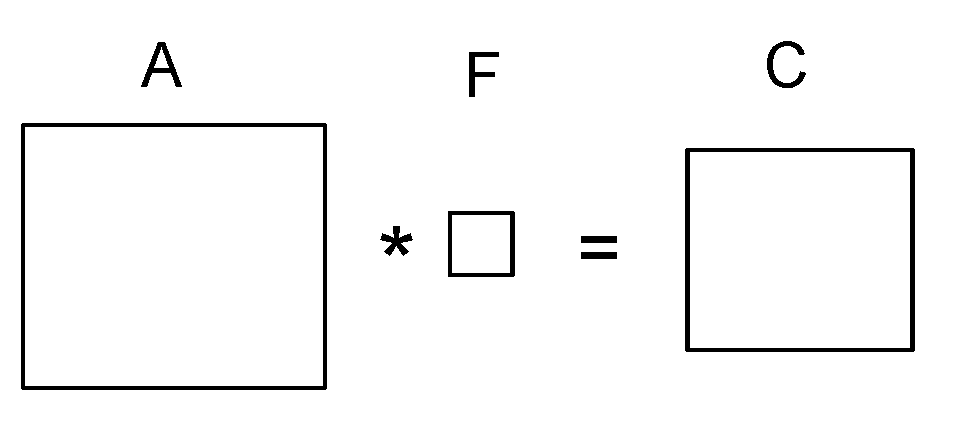
\includegraphics[width=\textwidth]{Conv-single}
}
\only<2->{
\begin{displaymath}
C(i, j) = \sum^{x = 0}_{m-1} \sum^{y = 0}_{n-1} A(x + i, y + j) F(x, y)
\end{displaymath}
\begin{itemize}
\item $(m, n)$ is the size of the filter.
\end{itemize}
}
\end{overlayarea}
Where $A$ is the input channel, $F$ is the filter and $C$ is the output channel.
\end{frame}

\begin{frame}
The basic convolution operation with multiple outputs
\begin{overlayarea}{\textwidth}{5.6cm}
\only<1>{
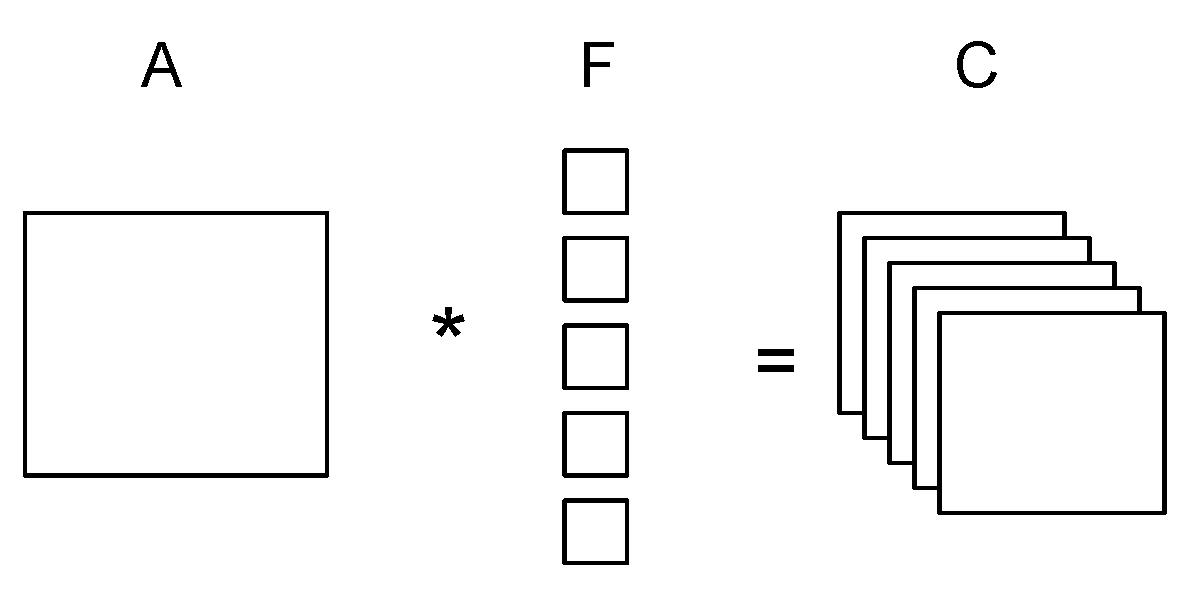
\includegraphics[width=\textwidth]{Conv-mout}
}
\only<2->{
\begin{displaymath}
C_{o}(i, j) = \sum^{x = 0}_{m-1} \sum^{y = 0}_{n-1} A(x + i, y + j) F_{o}(x, y)
\end{displaymath}
\begin{itemize}
\item $(m, n)$ is the size of the filters.
\item $o$ is the output channel.
\end{itemize}
}
\end{overlayarea}
where $A$ is the input channel, $F$ are the filters and $C$ are output channels.
\end{frame}

\begin{frame}
The basic convolution operation with multiple inputs
\begin{overlayarea}{\textwidth}{5.6cm}
\only<1>{
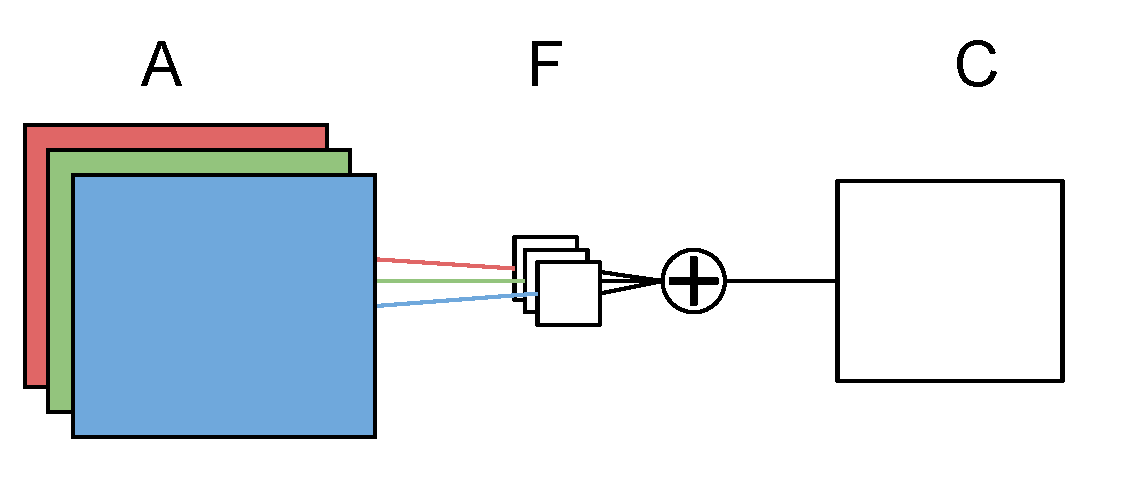
\includegraphics[width=\textwidth]{Conv-min}
}
\only<2->{
\begin{displaymath}
C(i, j) = \sum^{k=0}_l \sum^{x = 0}_{m-1} \sum^{y = 0}_{n-1} A_{k}(x + i, y + j) F_{k}(x, y)
\end{displaymath}
\begin{itemize}
\item $(m, n)$ is the size of the filters.
\item $k$ is the input channel.
\item $l$ is the number of input channels.
\end{itemize}
}
\end{overlayarea}
where $A$ are the input channels, $F$ is the filter bank and $C$ is the output channel.
\end{frame}

\begin{frame}
The basic convolution operation with multiple inputs and outputs
\begin{overlayarea}{\textwidth}{5.6cm}
\only<1>{
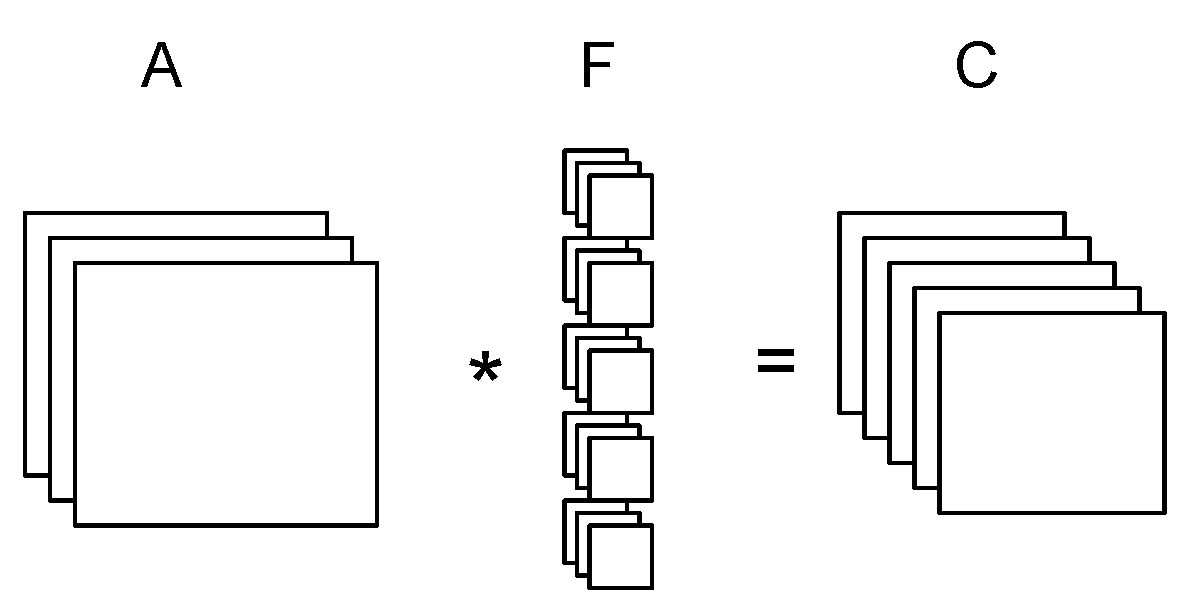
\includegraphics[width=\textwidth]{Conv-basic}
}
\only<2->{
\begin{displaymath}
C_{o}(i, j) = \sum^{k=0}_{l-1} \sum^{x = 0}_{m-1} \sum^{y = 0}_{n-1} A_{k}(x + i, y + j) F_{ko}(x, y)
\end{displaymath}
\begin{itemize}
\item $(m, n)$ is the size of the filters.
\item $o$ is the output channel.
\item $k$ is the input channel.
\item $l$ is the number of input channels.
\end{itemize}
}
\end{overlayarea}
where $A$ are the input channels, $F$ are the filter banks and $C$ are the output channels.
\end{frame}

\begin{frame}
The basic convolution operation with batches
\begin{overlayarea}{\textwidth}{5.6cm}
\only<1>{
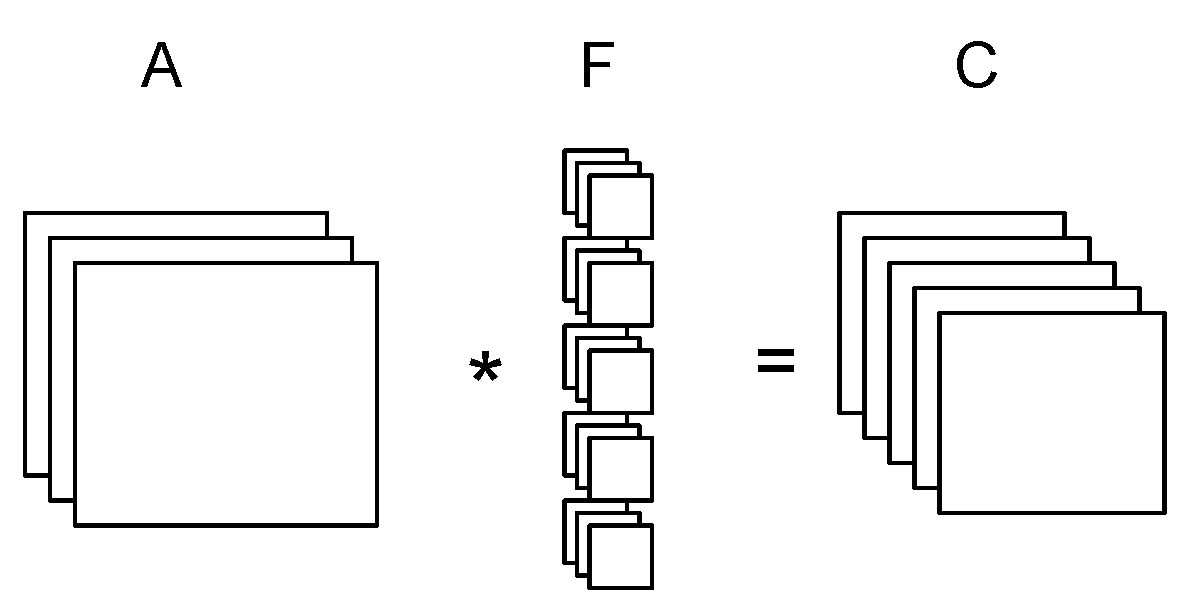
\includegraphics[width=\textwidth]{Conv-basic}
}
\only<2->{
\begin{displaymath}
C_{bo}(i, j) = \sum^{k=0}_{l-1} \sum^{x = 0}_{m-1} \sum^{y = 0}_{n-1} A_{bk}(x + i, y + j) F_{ko}(x, y)
\end{displaymath}
\begin{itemize}
\item $(m, n)$ is the size of the filters.
\item $o$ is the output channel.
\item $k$ is the input channel.
\item $l$ is the number of input channels.
\item $b$ is the batch.
\end{itemize}
}
\end{overlayarea}
where $A$ are the input channels, $F$ are the filter banks and $C$ are the output channels.
\end{frame}

% Definitions
\begin{frame}
Some vocabulary:
\begin{description}[filter banks]
\item[filter] what we call the smaller or "learned" 2D matrix in a traditional convolution.
\item[channel] what we call input or output 2D matrices in a traditional convolution.  Sometimes called \term{feature map}.
\item[filter bank] group of filters whose convolution output will be summed to form one output channel.  Sometimes called \term{filter stack}.
\end{description}
\end{frame}

% Technical considerations
\begin{frame}
Memory layout for images: 'bc01'

\begin{itemize}
\item first dimension is the batch ('b')
\item second dimension is the channel ('c')
\item last two dimensions are the data ('0', '1')
\end{itemize}

Memory layout for filters: 'nc01'

\begin{itemize}
\item first dimension is the output channel ('n')
\item second dimension is the input channel ('c')
\item last two dimensions are the data ('0', '1')
\end{itemize}

\ \\

\uncover<2->{Some other packages may use different conventions.}
\end{frame}

\section{Pooling}

\begin{frame}
Basic pooling operation
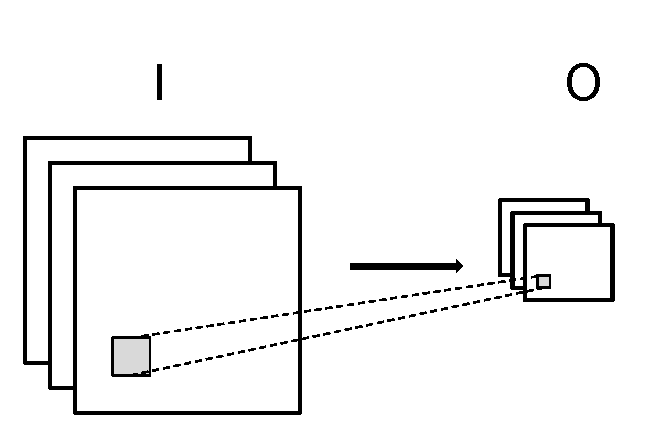
\includegraphics[width=\textwidth]{Pool-max}
\end{frame}

\begin{frame}
Max Pooling
\begin{displaymath}
O_k(i, j) = \max_{\substack{0 \leq x < m \\ 0 \leq y < n}} I_k(x + i, y + j)
\end{displaymath}
Average Pooling
\begin{displaymath}
O_k(i, j) = \frac{1}{mn}\sum^{x = 0}_{m - 1} \sum^{y = 0}_{n - 1} I_k(x + i, y + j)
\end{displaymath}
\begin{itemize}
\item $k$ is the channel.
\item $(m, n)$ is the size of the filters.
\end{itemize}
\end{frame}

\end{document}